% Provenance (never printed): see sources/outline_sources.md (Year 2: the Himalaya and Tibet;
% the Andes; crustal thickening and plateaus). Himalayan units, thrusts and rates after Lave
% and Avouac (2000), Ader et al. (2012), Cattin et al. (2001), Dong et al. (2026, STDS);
% Asian extrusion after Jiao et al. (2023); Tibetan rifts after Wang et al. (2021); Central
% Andes after Gerbault et al. (2005); flat slabs after Gauthier et al. (2024). Relief from
% ETOPO1 (figdata/bachelor-2/plateaus.py); plate velocities from NNR-MORVEL56 (Book 2 ledger
% row nnr56:poles). Exercise and problem values in the Book 4 scratch calculator
% calc/ch14.py.
\chapter{टक्कर-पट्टियाँ और एंडीज़-प्रकार की पट्टियाँ: एक तुलना}\label{ch:b2:himalaya-andes}

पृथ्वी पर दो पठार सैकड़ों किलोमीटर तक चार किलोमीटर से अधिक ऊँचे खड़े हैं।
तिब्बत वहाँ उठा जहाँ भारत एशिया से टकराया, यानी दो महाद्वीप उनके बीच के महासागर के लुप्त होने के बाद
मिले। आल्टिप्लानो वहाँ उठा जहाँ एक महासागरीय प्लेट, नाज़्का प्लेट, अब भी दक्षिण अमेरिका के
नीचे सरकती है, और कोई महाद्वीप आया ही नहीं। दो भिन्न इंजनों ने दो
मिलते-जुलते भू-आकार बनाए। यह अध्याय दोनों पट्टियों को खोलकर देखता है, मापता है कि उनकी भूपर्पटी कितनी मोटी
हुई है और क्यों, और पूछता है कि उन्हें और ऊँचा होने से क्या रोकता है।
% ledger: lave00:setting, gerbault05:andes, data:b4-etopo-tibet, data:b4-etopo-andes

\begin{recall}
\textbf{पुस्तक 2 (उच्च माध्यमिक) से}: महाद्वीपीय टक्कर और सीवन; भारत का
उत्तर की ओर बहाव, उसका धीमा होना और टक्कर की विवादित आयु; तिब्बत का पठार, लगभग
\qty{4600}{m} ऊँचा, लगभग \qty{70}{km} मोटी भूपर्पटी पर। \textbf{पुस्तक 3 (स्नातक वर्ष 1) से}:
एयरी समस्थिति और बूगेर पट्टी; सक्रिय किनारे, क्षेपित होता स्लैब, ज्वालामुखी चाप और
चाप--खाई अंतराल; कोणीय वेगों से प्लेट-वेग; बायरली का नियम; आघूर्ण
परिमाण। \textbf{\cref{ch:b2:crustal-melting} से}: हिमालय के \omterm{def:b2:crustal-melting:leucogranite}{ल्यूकोग्रेनाइट}।
\textbf{\cref{ch:b2:alpine-orogen} से}: \omterm{def:b2:alpine-orogen:orogen}{पर्वतजनक पट्टी}, \omterm{def:b2:alpine-orogen:nappes}{नैप}, \omterm{def:b2:alpine-orogen:decollement}{डेकोलमां}, पतली- और
\omterm{def:b2:alpine-orogen:skin}{मोटी-त्वचा विवर्तनिकी}, \omterm{def:b2:alpine-orogen:ftb}{वलन--अधिक्षेप पट्टी}, \omterm{def:b2:alpine-orogen:foreland}{अग्रभूमि द्रोणी}, \omterm{def:b2:alpine-orogen:balanced}{संतुलित अनुप्रस्थ काटें}।
\end{recall}

\begin{definition}[टक्कर-पट्टी; एंडीज़-प्रकार की पर्वतजनक पट्टी]\label{def:b2:himalaya-andes:types}
\emph{टक्कर-पट्टी}\index{टक्कर-पट्टी} वह \omterm{def:b2:alpine-orogen:orogen}{पर्वतजनक पट्टी} है जो दो महाद्वीपीय किनारों के
अभिसरण से, उनके बीच के महासागर के खप जाने के बाद, बनती है; उसकी अक्ष एक सीवन होती है।
\emph{एंडीज़-प्रकार की पर्वतजनक पट्टी}\index{एंडीज़-प्रकार की पर्वतजनक पट्टी} वह \omterm{def:b2:alpine-orogen:orogen}{पर्वतजनक पट्टी} है जो किसी महासागर--महाद्वीप क्षेपण-क्षेत्र की
ऊपरी प्लेट पर बनती है, जबकि उसके नीचे क्षेपण जारी रहता है; उसकी अक्ष
एक ज्वालामुखी चाप होती है।
\end{definition}


\section{भारत बनाम एशिया}\label{sec:b2:himalaya-andes:himalaya}

भारत लगभग 50 मिलियन वर्ष पहले सिंधु--त्सांगपो सीवन के अनुदिश यूरेशिया के दक्षिणी किनारे से मिला,
जिसे सिंधु--यारलुंग सीवन भी कहते हैं; सटीक तिथि पर अब भी बहस है, जैसा
पुस्तक 2 ने दिखाया। अभिसरण रुका नहीं। आज भारत और एशिया एक-दूसरे की ओर
लगभग \qty{40}{mm} प्रति वर्ष की दर से बढ़ रहे हैं; NNR-MORVEL56 प्लेट-प्रतिरूप के कोणीय वेगों से,
भारत यूरेशिया के सापेक्ष \qty{45}{mm} प्रति वर्ष की दर से \ang{28}~N, \ang{85}~E पर चलता है, उत्तर से
\ang{22} पूर्व की दिशा में। उस गति का केवल एक भाग हिमालय में खपता है। नेपाल के आर-पार,
GPS स्टेशन भारत और दक्षिणी तिब्बत को मध्य और पूर्व में $17.8 \pm \qty{0.5}{mm}$ प्रति वर्ष तथा
पश्चिम में $20.5 \pm \qty{1}{mm}$ प्रति वर्ष की दर से अभिसरित होते दिखाते हैं: कुल का लगभग आधा। शेष
तिब्बत और बाक़ी एशिया पर फैला है।
% ledger: lave00:setting, najman21:collision-age, jiao23:extrusion, nnr56:poles, ader12:rates, ader12:mht
% values (plateaus.py): v_india_eurasia 44.99 mm/yr, azimuth 21.65

नीचे के मानचित्र दोनों पट्टियों को एक-सी समोच्च रेखाओं के साथ दिखाते हैं, और वे पट्टियाँ भी जिनके अनुदिश यह
अध्याय उन्हें काटता है।

\begin{omfigure}
\centering
% ledger: data:b4-etopo-tibet, data:b4-etopo-andes
\begin{tikzpicture}
\begin{axis}[name=tib, scale only axis, width=8.0cm, height=4.8cm, xmin=75, xmax=100,
  ymin=25, ymax=40, xlabel={देशांतर (\unit{\degree} E)}, ylabel={अक्षांश (\unit{\degree} N)},
  tick label style={font=\scriptsize}, label style={font=\small}, xtick={75,80,...,100},
  ytick={25,30,...,40}, title={\small हिमालय और तिब्बत}]
\addplot[omThm!35, line width=0.3pt] table[x=lon, y=lat] {figdata/out/bachelor-2-plateaus-tc2000.dat};
\addplot[omThm!90!black, line width=0.4pt] table[x=lon, y=lat] {figdata/out/bachelor-2-plateaus-tc4000.dat};
\draw[black, densely dashed, line width=0.9pt] (axis cs:86,25) rectangle (axis cs:90,40);
\node[font=\scriptsize, fill=white, fill opacity=0.85, text opacity=1, inner sep=1pt] at (axis cs:80,26.2) {गंगा का मैदान};
\node[font=\scriptsize, fill=white, fill opacity=0.85, text opacity=1, inner sep=1pt] at (axis cs:94.5,33.5) {तिब्बत का पठार};
\node[font=\scriptsize, fill=white, fill opacity=0.85, text opacity=1, inner sep=1pt] at (axis cs:83,39.2) {तारिम};
\end{axis}
\begin{axis}[at={(tib.east)}, anchor=west, xshift=1.6cm, scale only axis, width=3.6cm,
  height=4.8cm, xmin=-75, xmax=-60, ymin=-30, ymax=-10,
  xlabel={देशांतर (\unit{\degree})}, tick label style={font=\scriptsize},
  label style={font=\small}, xtick={-75,-70,-65,-60}, ytick={-30,-25,...,-10},
  title={\small मध्य एंडीज़}]
\addplot[blue!60!black, line width=0.45pt] table[x=lon, y=lat] {figdata/out/bachelor-2-plateaus-ac0.dat};
\addplot[omThm!35, line width=0.3pt] table[x=lon, y=lat] {figdata/out/bachelor-2-plateaus-ac2000.dat};
\addplot[omThm!90!black, line width=0.4pt] table[x=lon, y=lat] {figdata/out/bachelor-2-plateaus-ac4000.dat};
\draw[black, densely dashed, line width=0.9pt] (axis cs:-75,-21) rectangle (axis cs:-60,-19);
\node[font=\scriptsize, fill=white, fill opacity=0.85, text opacity=1, inner sep=1pt] at (axis cs:-73,-25) {प्रशांत};
\end{axis}
\end{tikzpicture}
\par\smallskip{\small ETOPO1 से दोनों पट्टियों का उच्चावच, हर बिंदु \qty{0.1}{\degree}
दूर: \qty{2000}{m} (हल्की) और \qty{4000}{m} (गहरी) पर समोच्च रेखाएँ, और दाईं ओर
तटरेखा। दाईं ओर अक्षांश विषुवत के दक्षिण में ऋणात्मक हैं, और देशांतर
ग्रीनविच के पश्चिम में ऋणात्मक। धराशायी आयत आगे के प्रोफ़ाइलों की पट्टियाँ हैं: हिमालय और तिब्बत के आर-पार \qtyrange{86}{90}{\degree} E,
मध्य एंडीज़ के आर-पार \qtyrange{19}{21}{\degree} S।}
\end{omfigure}

\subsection{इकाइयाँ और अधिक्षेप}

गंगा के मैदान से उत्तर की ओर, हिमालय का एक आर-पार भ्रमण अधिक्षेप-चादरों के एक ढेर को पार करता है
जो भारत के उत्तरी किनारे से काटी गई हैं, और उन भ्रंशों से अलग हैं जो पर्वतमाला की पूरी लंबाई में चलते हैं।
\begin{itemize}
\item \emph{सिंधु-गंगा अग्रगर्त} हिमालय की \omterm{def:b2:alpine-orogen:foreland}{अग्रभूमि द्रोणी} है; वह पर्वतमाला से अपरदित
मलबे का एक भाग रोक लेती है।
\item \emph{उप-हिमालय}, यानी शिवालिक पहाड़ियाँ, उसी द्रोणी के \omterm{def:b2:alpine-orogen:foreland}{मोलास} से बनी है,
यानी उत्तर मायोसीन से प्लाइस्टोसीन आयु के मृत्तिकाश्म से संगुटिकाश्म तक, 3500 से \qty{5500}{m} मोटे,
जो 14 और \qty{1}{Ma} के बीच जमे, फिर पर्वतमाला के अग्र पर खुरचे गए और एक
\omterm{def:b2:alpine-orogen:decollement}{डेकोलमां} के ऊपर वलित हुए: एक पतली-त्वचा \omterm{def:b2:alpine-orogen:ftb}{वलन--अधिक्षेप पट्टी}। उसका दक्षिणी किनारा \emph{मुख्य अग्र
अधिक्षेप} (MFT) है।
\item \emph{लघु हिमालय}, मध्यम \omterm{def:b2:metamorphic-facies:metamorphism}{कायांतरण} श्रेणी की चट्टानें, नीचे
\emph{मुख्य सीमा अधिक्षेप} (MBT) और ऊपर \emph{मुख्य केंद्रीय अधिक्षेप} (MCT) के बीच स्थित है।
\item MCT के ऊपर \emph{बृहत् हिमालयी अनुक्रम} (उच्च हिमालय)
उच्च-श्रेणी की कायांतरित चट्टानों से बना है, आंशिक रूप से गलित: \cref{ch:b2:crustal-melting} के
\omterm{def:b2:crustal-melting:migmatite}{मिग्मेटाइट} और \omterm{def:b2:crustal-melting:leucogranite}{ल्यूकोग्रेनाइट}, जो टक्कर के लगभग 30 मिलियन वर्ष बाद गले।
\item \emph{टेथिस हिमालयी अनुक्रम}, भारत के पुराने निष्क्रिय किनारे के अकायांतरित या दुर्बल रूप से कायांतरित
अवसाद, बृहत् हिमालयी अनुक्रम पर
\emph{दक्षिण तिब्बत विलगन तंत्र} (STDS) के अनुदिश टिका है, जो पर्वतमाला के महान पूर्व--पश्चिम भ्रंश-मंडलों में
अकेला सामान्य भ्रंश है, \qty{2000}{km} से अधिक लंबा।
\item उनके उत्तर में सीवन आती है, और उसके पार दक्षिणी तिब्बत की एशियाई भूपर्पटी।
\end{itemize}
% ledger: lave00:setting, lave00:siwaliks, weinberg16:himalaya, dong26:stds

भ्रंश दक्षिण की ओर क्रमशः नए होते जाते हैं। विरूपण-अग्र दक्षिण की ओर खिसका, क्योंकि एक के बाद एक अधिक्षेप ने
कार्य सँभाला, कांगमार अधिक्षेप से MCT तक, फिर MBT, और अब MFT, जो मध्य
नेपाल में उप-हिमालय की अकेली सक्रिय संरचना है। यह वही बाहर की ओर
स्थानांतरण है जो \cref{ch:b2:alpine-orogen} के आल्प्स में था, यहाँ उन चट्टानों में लिखा जो अब भी
चल रही हैं। STDS एक आश्चर्य जोड़ता है: एक सामान्य भ्रंश, यानी विस्तारण, ऐसी पर्वतमाला के भीतर जो
छोटी की जा रही है। यह दिखाता है कि संपीडन और विस्तारण एक ही \omterm{def:b2:alpine-orogen:orogen}{पर्वतजनक पट्टी} में एक साथ काम कर सकते हैं,
भिन्न स्तरों पर, और इसने बृहत् हिमालयी अनुक्रम की गर्म चट्टानों को पर्वतमाला की जड़ से
ऊपर लाने में सहायता की।
% ledger: lave00:setting, lave00:mft-rate, dong26:stds

\subsection{पर्वतमाला के नीचे एक भ्रंश}

सतह के अधिक्षेप एक अकेले, मंद नत भ्रंश में जड़ जमाते हैं, यानी \emph{मुख्य
हिमालयी अधिक्षेप} (MHT), जिसके अनुदिश भारतीय प्लेट पर्वतमाला के नीचे धकेली जाती है। यह
MFT पर सतह तक पहुँचता है, लघु हिमालय के नीचे एक समतल भाग के रूप में चलता है, उच्च हिमालय के अग्र पर
एक रैंप में खड़ा हो जाता है, और दक्षिणी तिब्बत के नीचे उत्तर की ओर जारी रहता है। होलोसीन के दौरान
शिवालिक के आर-पार नदी-वेदिकाओं का वलन MFT पर $21 \pm \qty{1.5}{mm}$ प्रति वर्ष
लघुकरण अंकित करता है, जो पूरी पर्वतमाला के आर-पार की भूगणितीय दर के बराबर है। MHT
सतह से नति की दिशा में लगभग \qty{100}{km} तक, 15 से \qty{20}{km} गहराई पर, जकड़ा हुआ है; आगे
उत्तर में वह मंद सरकन करता है। जकड़ा भाग अभिसरण को प्रत्यास्थ विकृति के रूप में संचित करता है और उसे
बड़े भूकंपों में लौटाता है, जैसे 1950 का असम भूकंप, जिसका आघूर्ण परिमाण लगभग~8.5 था।
% ledger: ader12:mht, lave00:setting, lave00:mft-rate, ader12:quakes

\begin{omfigure}
\centering
\begin{tikzpicture}[x=0.6cm, y=0.5cm, font=\scriptsize]
% Indian crust below the MHT and the foredeep
\fill[gray!15] (0,-0.4) -- (5,-0.8) -- (12,-1.6) -- (14,-3.2) -- (24,-4.2) -- (24,-8.5) -- (0,-5.5) -- cycle;
% mantle
\fill[gray!35] (0,-5.5) -- (24,-8.5) -- (24,-9.3) -- (0,-6.3) -- cycle;
% foredeep
\fill[yellow!35] (0,0) -- (4,0) -- (5,-0.8) -- (0,-0.4) -- cycle;
% Siwaliks
\fill[orange!35] (4,0) -- (5,0.6) -- (6.5,0.8) -- (7.6,-1.1) -- (5,-0.8) -- cycle;
% Lesser Himalaya
\fill[green!20] (6.5,0.8) -- (8.5,1.3) -- (11,2.0) -- (13,-2.4) -- (12,-1.6) -- (7.6,-1.1) -- cycle;
% Greater Himalayan sequence
\fill[omThm!35] (11,2.0) -- (12.5,3.6) -- (13.5,4.2) -- (15,3.6) -- (19.53,0.2) -- (20.2,-3.82)
  -- (14,-3.2) -- (13,-2.4) -- cycle;
% Tethyan Himalayan sequence
\fill[cyan!20] (15,3.6) -- (17,3.5) -- (19,3.4) -- (19.53,0.2) -- cycle;
% Asian crust
\fill[orange!15] (19,3.4) -- (24,3.4) -- (24,-4.2) -- (20.2,-3.82) -- cycle;
% leucogranites
\fill[pink!70!red!45] (14.2,2.2) ellipse (0.45 and 0.35);
\fill[pink!70!red!45] (16.6,1.0) ellipse (0.4 and 0.3);
% surface
\draw[line width=0.5pt] (0,0) -- (4,0) -- (5,0.6) -- (6.5,0.8) -- (8.5,1.3) -- (11,2.0) -- (12.5,3.6)
  -- (13.5,4.2) -- (15,3.6) -- (17,3.5) -- (19,3.4) -- (24,3.4);
% faults
\draw[thick] (6.5,0.8) -- (7.6,-1.1);
\draw[thick] (11,2.0) -- (13,-2.4);
\draw[thick, densely dashed] (15,3.6) -- (19.53,0.2);
\draw[thick] (19,3.4) -- (20.2,-3.82);
% MHT
\draw[very thick, red!70!black] (4,0) -- (5,-0.8) -- (12,-1.6) -- (14,-3.2) -- (24,-4.2);
\node[red!70!black, anchor=north] at (8.8,-1.25) {MHT, जकड़ा समतल भाग};
\node[red!70!black, anchor=north east] at (13.2,-2.6) {रैंप};
\node[red!70!black, anchor=north] at (19.5,-4.0) {MHT, मंद सरकन};
% Moho
\draw[dashed] (0,-5.5) -- (24,-8.5);
\node[anchor=south west] at (0.2,-5.45) {भारतीय मोहो};
\node at (12,-5.6) {भारतीय भूपर्पटी};
\node at (16,-7.9) {प्रावार};
% unit labels
\node[anchor=south] at (1.8,0.05) {अग्रगर्त};
\node at (5.6,0.05) {शिवा॰};
\node at (9.3,0.5) {लघु हिमालय};
\node[align=center] at (15.6,-0.9) {बृहत् हिमालयी\\अनुक्रम};
\node[align=center] at (18.1,2.65) {टेथिस\\हिमालय};
\node at (21.8,0.2) {एशियाई भूपर्पटी};
% fault labels
\node[anchor=south, font=\scriptsize\bfseries] (mft) at (3.2,1.6) {MFT};
\draw[->] (mft.south) -- (3.95,0.1);
\node[anchor=south, font=\scriptsize\bfseries] (mbt) at (5.9,2.3) {MBT};
\draw[->] (mbt.south) -- (6.5,0.95);
\node[anchor=south, font=\scriptsize\bfseries] (mct) at (10.2,3.6) {MCT};
\draw[->] (mct.south) -- (11.0,2.15);
\node[anchor=south, font=\scriptsize\bfseries] (stds) at (16.6,5.0) {STDS};
\draw[->] (stds.south) -- (15.8,3.1);
\node[anchor=south, font=\scriptsize\bfseries] (sut) at (20.6,5.0) {सीवन};
\draw[->] (sut.south) -- (19.2,2.4);
\draw[-{Latex[length=2mm]}] (1.2,2.4) -- (0.2,2.4);
\node[anchor=south] at (0.7,2.4) {\omnameCompassS};
\draw[-{Latex[length=2mm]}] (22.8,5.0) -- (23.8,5.0);
\node[anchor=south] at (23.3,5.0) {\omnameCompassN};
\end{tikzpicture}
\par\smallskip{\small नेपाल के हिमालय के आर-पार एक योजनामूलक काट (पैमाने के बिना)।
अधिक्षेप MCT से MBT और MFT की ओर दक्षिण में क्रमशः नए होते हैं, और सभी मुख्य
हिमालयी अधिक्षेप (MHT) में जड़ जमाते हैं, जो लघु हिमालय के नीचे जकड़ा है और दक्षिणी
तिब्बत के नीचे मंद सरकन करता है; STDS (धराशायी) एक सामान्य भ्रंश है। बृहत् हिमालयी
अनुक्रम में \omterm{def:b2:crustal-melting:leucogranite}{ल्यूकोग्रेनाइट} (गुलाबी); शिवा॰, शिवालिक। भारतीय मोहो पर्वतमाला के नीचे उत्तर की ओर गहरा होता जाता है।}
\end{omfigure}
% ledger: lave00:setting, ader12:mht, dong26:stds, weinberg16:himalaya, cattin01:crust

बृहत् हिमालयी अनुक्रम, जो गहराई पर आंशिक रूप से गलित था, नीचे एक अधिक्षेप और ऊपर एक सामान्य भ्रंश के
बीच कैसे आ खड़ा हुआ? एक परिकल्पना, \emph{वाहिका-प्रवाह}, के अनुसार गर्म,
दुर्बल मध्य भूपर्पटी दोनों अपरूपण-मंडलों के बीच दक्षिण की ओर बाहर बहती है, और वहाँ सतह की ओर खिंचती है
जहाँ अपरदन सबसे तेज़ है। यह एक परिकल्पना है: हिमालय और तिब्बत के निर्माण में वाहिका-प्रवाह, निपात
और विस्तरीकरण का हिस्सा अब भी विवादित है।
% ledger: gerbault05:delamination, jiao23:extrusion, dong26:stds

पर्वतमाला मुक्त रूप से नहीं तैरती। नेपाल के आर-पार गुरुत्व-प्रोफ़ाइल गंगा के मैदान से तिब्बत तक
बूगेर विसंगति को लगभग $-40$ से \qty{-500}{mGal} तक गिरते दिखाते हैं।
पर्वतमाला से दूर स्थानीय एयरी समस्थिति लागू होती है; उसके निकट अग्रभूमि अति-प्रतिपूरित है और ऊँची
पर्वतमाला अल्प-प्रतिपूरित: भारतीय प्लेट पर्वतों के भार के नीचे किसी धरन की तरह नीचे झुकी है
और अपनी ही दृढ़ता से उन्हें आंशिक रूप से थामे रखती है, एक क्षेत्रीय आलंब जिसका अध्ययन
पुस्तक 5 (स्नातक वर्ष 3) का विषय है।
% ledger: cattin01:crust

\begin{inthefield}[चलती हुई पर्वत-पट्टी को मापना]
हिमालय में एक भूगणित-दल स्थायी GPS स्टेशन लगाता है: आधारशैल पर या
कंक्रीट के खंभे पर बोल्ट से कसा एक ऐंटेना, एक रिसीवर, एक सौर पैनल, एक बैटरी। हर स्टेशन प्रतिदिन अपनी
स्थिति अंकित करता है। एक दिन की स्थिति मिलीमीटरों में बिखरती है, और यह रव पूरी तरह
यादृच्छिक नहीं है: यह हफ़्तों और ऋतुओं में भटकता है। इसलिए दल वर्षों की दैनिक स्थितियों पर एक सीधी रेखा
बिठाने से पहले रव का प्रतिरूप बनाता है, श्वेत और रंगीन दोनों; ढलान
स्टेशन का दीर्घकालिक वेग है, एक ईमानदार अनिश्चितता के साथ। नेपाल के आर-पार, लगभग बीस वर्षों तक देखे गए
लगभग तीस स्टेशन ऐसे वेग दिखाते हैं जो लगभग सौ किलोमीटर चौड़ी एक पट्टी में भारत के वेग से दक्षिणी तिब्बत के वेग तक
गिरते हैं, ठीक उस स्थान के ऊपर जहाँ MHT जकड़ी अवस्था से
मंद सरकन में बदलता है।
\end{inthefield}
% ledger: ader12:rates, ader12:mht

\section{तिब्बत, ऊँचा पठार}\label{sec:b2:himalaya-andes:tibet}

\begin{definition}[पर्वतजनक पठार]\label{def:b2:himalaya-andes:plateau}
\emph{पर्वतजनक पठार}\index{पर्वतजनक पठार} किसी \omterm{def:b2:alpine-orogen:orogen}{पर्वतजनक पट्टी} का सैकड़ों
किलोमीटर चौड़ा वह क्षेत्र है जहाँ सतह औसतन ऊँची और लगभग समतल खड़ी है, और उसका उच्चावच
आसपास की निचली भूमियों से उसकी ऊँचाई की तुलना में छोटा है।
\end{definition}

\begin{definition}[भूपर्पटीय स्थूलन]\label{def:b2:himalaya-andes:thickening}
\emph{भूपर्पटीय स्थूलन}\index{भूपर्पटीय स्थूलन} (भूपर्पटी का मोटा होना) किसी क्षेत्र की भूपर्पटी की मोटाई में
वृद्धि है, जो स्वयं भूपर्पटी के लघुकरण से, नीचे से \omterm{def:b2:magma-emplacement:magma}{मैग्मा} के जुड़ने से, या
उसके नीचे अधिक्षेपित होती या बहती अन्य भूपर्पटी से होती है।
\end{definition}

नीचे के प्रोफ़ाइल दोनों पठारों को काटते हैं। पट्टी \qtyrange{86}{90}{\degree} E के अनुदिश माध्य
ऊँचाई गंगा के मैदान पर लगभग \qty{70}{m} से बढ़कर लगभग \qty{5000}{m} तक पहुँचती है, और यह
\qty{170}{km} से कम दूरी में; फिर वह \qty{3000}{m} से ऊपर \qty{1180}{km} तक बनी रहती है, \ang{27.6}~N से
\ang{38.2}~N तक, \qty{4830}{m} के माध्य के साथ। उसके नीचे भूपर्पटी 70 से \qty{75}{km} मोटी है,
जो गंगा के मैदान के दक्षिण में भारतीय भूपर्पटी के 35 से \qty{40}{km} की दोगुनी है।
% ledger: data:b4-etopo-tibet, cattin01:crust, karplus:tibet-moho
% values (plateaus.py): tibet_plateau 27.6-38.2 N, width 1178.6 km, mean 4828.99 m

\begin{omfigure}
\centering
% ledger: data:b4-etopo-tibet, data:b4-etopo-andes
\begin{tikzpicture}
\begin{groupplot}[group style={group size=1 by 2, vertical sep=1.5cm},
  width=0.95\linewidth, height=4.6cm, xmin=0, xmax=1670,
  ylabel={ऊँचाई (\unit{m})}, tick label style={font=\scriptsize},
  label style={font=\small}, legend style={font=\scriptsize, fill=white}]
\nextgroupplot[ymin=0, ymax=9500, xlabel={\ang{25}~N से उत्तर की ओर दूरी,
  \qtyrange{86}{90}{\degree} E के अनुदिश (\unit{km})}, legend columns=3,
  legend style={at={(0.5,1.04)}, anchor=south, draw=none}]
\addplot[gray, line width=0.4pt] table[x=km, y=max_m] {figdata/out/bachelor-2-plateaus-tswath.dat};
\addplot[omThm, line width=1.1pt] table[x=km, y=mean_m] {figdata/out/bachelor-2-plateaus-tswath.dat};
\addplot[gray!60, line width=0.4pt] table[x=km, y=min_m] {figdata/out/bachelor-2-plateaus-tswath.dat};
\addplot[black, dashed, line width=0.7pt, forget plot] coordinates {(289.1,4829) (1467.7,4829)};
\legend{अधिकतम, माध्य, न्यूनतम}
\node[font=\scriptsize, anchor=south] at (axis cs:880,6600) {पठार का माध्य \qty{4830}{m}};
\node[font=\scriptsize, anchor=south west] at (axis cs:10,2600) {गंगा का मैदान};
\node[font=\scriptsize, anchor=south] at (axis cs:1625,2600) {तारिम};
\nextgroupplot[ymin=-9000, ymax=9000, xmax=1570, xlabel={\ang{75}~W से पूर्व की ओर दूरी,
  \qtyrange{19}{21}{\degree} S के अनुदिश (\unit{km})}]
\addplot[gray, line width=0.4pt] table[x=km, y=max_m] {figdata/out/bachelor-2-plateaus-aswath.dat};
\addplot[omThm, line width=1.1pt] table[x=km, y=mean_m] {figdata/out/bachelor-2-plateaus-aswath.dat};
\addplot[gray!60, line width=0.4pt] table[x=km, y=min_m] {figdata/out/bachelor-2-plateaus-aswath.dat};
\addplot[black, dashed, line width=0.7pt] coordinates {(616.4,3761) (1055.3,3761)};
\addplot[black!50, line width=0.3pt] coordinates {(0,0) (1570,0)};
\node[font=\scriptsize, anchor=south] at (axis cs:835,5200) {पठार का माध्य \qty{3760}{m}};
\node[font=\scriptsize, anchor=south] at (axis cs:120,-3200) {प्रशांत};
\node[font=\scriptsize, anchor=west] at (axis cs:470,-7300) {खाई};
\node[font=\scriptsize, anchor=south] at (axis cs:1400,700) {चाको मैदान};
\end{groupplot}
\end{tikzpicture}
\par\smallskip{\small ETOPO1 से दोनों पठारों के आर-पार पट्टी-प्रोफ़ाइल (बिंदु
\qty{0.1}{\degree} दूर): हर दूरी पर बिंदुओं की माध्य, अधिकतम और न्यूनतम ऊँचाई।
ऊपर: \qtyrange{86}{90}{\degree} E के अनुदिश हिमालय और तिब्बत। नीचे: मध्य एंडीज़,
\qtyrange{19}{21}{\degree} S के अनुदिश, प्रशांत तल और खाई से चाको मैदान तक।
धराशायी रेखाएँ पठार को, यानी उस खंड को जहाँ पट्टी-माध्य \qty{3000}{m} से ऊपर रहता है,
उस खंड की माध्य ऊँचाई पर चिह्नित करती हैं।}
\end{omfigure}
% values (plateaus.py): andes plateau -69.1 to -64.9, 438.8 km, mean 3761.03 m; trench -7666 m at -71.4

किसी दी हुई ऊँचाई के पठार के नीचे भूपर्पटी कितनी मोटी होनी चाहिए? पुस्तक 3 (स्नातक वर्ष 1)
का एयरी उत्तर इसे एक पंक्ति में देता है।

\begin{proposition}[माध्य ऊँचाई से भूपर्पटी की मोटाई]\label{prop:b2:himalaya-andes:airy}
मान लीजिए घनत्व $\rho_c$ की एक भूपर्पटी, जहाँ उसकी सतह समुद्र-तल पर है, वहाँ $H$ मोटी है, और
घनत्व $\rho_m$ के प्रावार पर स्थित है। यदि माध्य ऊँचाई $h$ के किसी पठार की प्रतिपूर्ति एयरी के ढंग से होती है, तो उसकी भूपर्पटी
है
\[
  T = H + h + h\,\frac{\rho_c}{\rho_m - \rho_c} = H + h\,\frac{\rho_m}{\rho_m - \rho_c} .
\]
विलोमतः, स्थूलन $\Delta T = T - H$ सतह को $h = \Delta T\,(\rho_m -
\rho_c)/\rho_m$ ऊपर उठाता है।
\end{proposition}

\begin{proof}
एयरी समस्थिति भूपर्पटी के सामान्य आधार के नीचे जड़ $r = h\rho_c/(\rho_m - \rho_c)$ देती है;
भूपर्पटी समुद्र-तल से ऊपर की ऊँचाई $h$, सामान्य मोटाई $H$ और जड़
$r$ में फैली है। जोड़ने पर, $h + h\rho_c/(\rho_m - \rho_c) = h\rho_m/(\rho_m - \rho_c)$। $h$ के लिए हल करने पर
विलोम मिलता है।
\end{proof}

पुस्तक 3 के घनत्वों, \qty{2700}{kg.m^{-3}} और \qty{3300}{kg.m^{-3}}, के साथ
गुणक $\rho_m/(\rho_m - \rho_c)$ का मान 5.5 है: पठार के हर किलोमीटर को \qty{5.5}{km}
अतिरिक्त भूपर्पटी चाहिए, जिसमें से \qty{4.5}{km} जड़ के रूप में, और \qty{10}{km} का हर स्थूलन केवल
\qty{1.8}{km} ऊँचाई खरीदता है। तिब्बत के लिए, $H = \qty{35}{km}$ और $h = \qty{4.8}{km}$ के साथ, $T = 35 +
5.5 \times 4.8 = \qty{61.4}{km}$, जो मापे गए 70 से \qty{75}{km} से कम है। इन
गोल घनत्वों के साथ एयरी जड़ को कम आँकता है; सघनतर भूपर्पटी, अतः मोहो पर कम घनत्व-अंतर,
उसी ऊँचाई के लिए गहरी जड़ माँगती है। और पर्वतमाला के निकट, जैसा ऊपर देखा, भार का एक भाग झुकी प्लेट वहन करती है,
किसी स्थानीय जड़ के बजाय।
% ledger: cattin01:crust
% values (plateaus.py): tibet_airy_T 61.4 km for h = 4.8

\begin{omfigure}
\centering
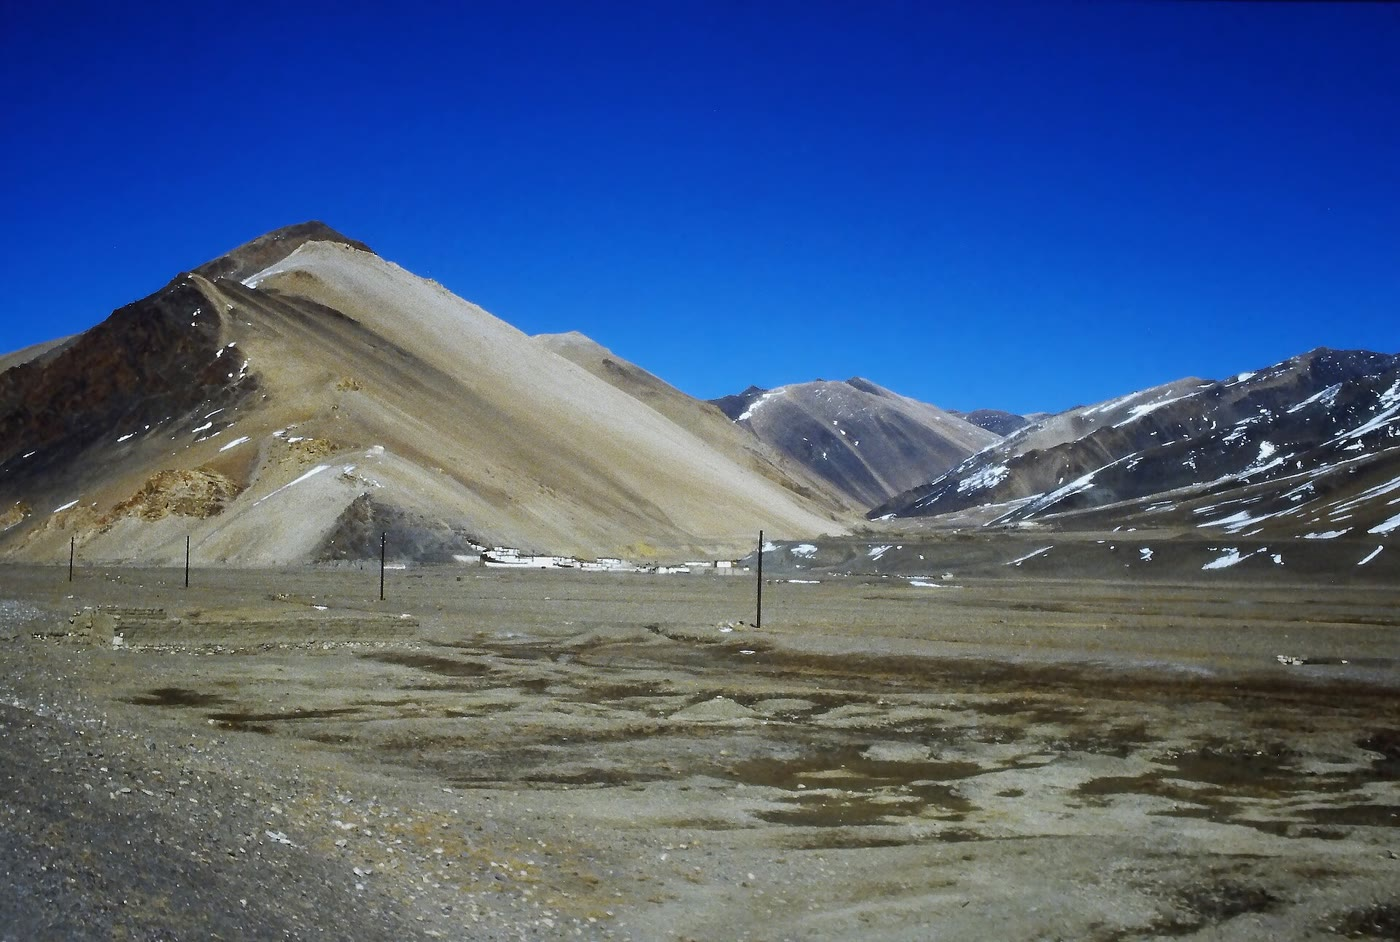
\includegraphics[width=0.66\linewidth]{images/book4/b2-14-tibet-plateau.jpg}
\par\smallskip{\small नेपाल और शिगात्से के बीच तिब्बत का पठार: बजरी और विरल चरागाह का एक समतल तल,
एक गाँव के साथ, मलबे से ढके नंगे पर्वतों के बीच, और यह सब समुद्र-तल से
चार किलोमीटर से अधिक ऊपर।
फ़ोटो: Jan Kranendonk, 1987, CC BY-SA 4.0।}
\end{omfigure}
% ledger: data:b4-etopo-tibet

\subsection{एक पठार का भार}

पठार अपने परिवेश पर भार डालता है। उसकी जड़ के आधार तक हर गहराई पर, पठार के नीचे का
स्तंभ पास की निचली भूमि के नीचे के स्तंभ से अधिक दाब में होता है;
केवल प्रतिपूर्ति-गहराई पर दोनों बराबर होते हैं। ऊँचा स्तंभ बाहर की ओर धकेलता है।

\begin{proposition}[किसी पठार की अतिरिक्त स्थितिज ऊर्जा]\label{prop:b2:himalaya-andes:gpe}
\cref{prop:b2:himalaya-andes:airy} की परिकल्पनाओं के अंतर्गत, गुरुत्व $g$ के साथ, सामान्य स्तंभ की तुलना में
पठार-स्तंभ के अतिरिक्त शिलास्थैतिक दाब का समाकल, पठार के शीर्ष
से उसकी जड़ $r$ के आधार पर स्थित प्रतिपूर्ति-गहराई तक, है
\[
  \Delta F = \rho_c g h \left(H + \frac{h}{2} + \frac{r}{2}\right) .
\]
यह प्रति इकाई क्षेत्रफल पठार-स्तंभ की अतिरिक्त गुरुत्वीय स्थितिज ऊर्जा है, और पठार के किनारे की
प्रति इकाई लंबाई पर वह बल जिससे पठार अपने
परिवेश पर धकेलता है।
\end{proposition}

\begin{proof}
गहराई $z$ को समुद्र-तल से नीचे की ओर मापिए। पठार-स्तंभ में दाब $p_1 =
\rho_c g (z + h)$ है, $z = -h$ से $L = H + r$ तक। सामान्य स्तंभ में यह समुद्र-तल के ऊपर शून्य,
भूपर्पटी में $\rho_c g z$, और नीचे $\rho_c g H + \rho_m g (z - H)$ है। अंतर $p_1
- p_0$ $z = -h$ पर 0 से बढ़कर समुद्र-तल पर $\rho_c g h$ हो जाता है; यह सामान्य भूपर्पटी में, जहाँ दोनों स्तंभ
भूपर्पटी हैं, यही मान रखता है; $z = H$ के नीचे यह रैखिक रूप से, प्रति मीटर
$(\rho_m - \rho_c) g$ से, घटता है, और $L$ पर शून्य हो जाता है क्योंकि $(\rho_m - \rho_c) r = \rho_c
h$। समाकल इस समलंब का क्षेत्रफल है: $\rho_c g h\,(h/2 + H + r/2)$। जब दोनों स्तंभ बग़ल में
पदार्थ का आदान-प्रदान करते हैं तब दाबों द्वारा किया गया कार्य
यही समाकल है, इसीलिए यह ऊर्जा और धक्के दोनों को मापता है।
\end{proof}

\begin{omfigure}
\centering
% figdata/bachelor-2/plateaus.py part pressure (h = 4.8 km, H = 35 km, 2700 and 3300 kg/m3)
\begin{tikzpicture}
\begin{axis}[width=0.62\linewidth, height=5.6cm, y dir=reverse, xmin=0, xmax=160, ymin=-12,
  ymax=60, xlabel={अतिरिक्त दाब $p_1 - p_0$ (\unit{MPa})}, ylabel={समुद्र-तल के नीचे गहराई
  (\unit{km})}, tick label style={font=\scriptsize}, label style={font=\small},
  xtick pos=bottom, ytick pos=left, clip=false]
\addplot[fill=omThm!20, draw=omThm, line width=1pt] table[x expr=\thisrow{p_high_MPa}-\thisrow{p_ref_MPa}, y=z_km] {figdata/out/bachelor-2-plateaus-pressure.dat} \closedcycle;
\draw[dashed] (axis cs:0,0) -- (axis cs:160,0);
\draw[dashed] (axis cs:0,35) -- (axis cs:160,35);
\draw[dashed] (axis cs:0,56.6) -- (axis cs:160,56.6);
\node[font=\scriptsize, anchor=north east] at (axis cs:160,0) {समुद्र-तल};
\node[font=\scriptsize, anchor=north east] at (axis cs:160,35) {सामान्य मोहो, $H$};
\node[font=\scriptsize, anchor=south east] at (axis cs:160,56.6) {जड़ का आधार, $H + r$};
\node[font=\scriptsize, anchor=west] at (axis cs:100,-8.4) {पठार का शीर्ष, $-h$};
\node[font=\scriptsize, align=center] at (axis cs:60,20) {क्षेत्रफल $= \Delta F$\\$\approx\qty{6.1e12}{N.m^{-1}}$};
\end{axis}
\end{tikzpicture}
\par\smallskip{\small सामान्य स्तंभ की तुलना में पठार-स्तंभ का अतिरिक्त शिलास्थैतिक दाब,
$h = \qty{4.8}{km}$, $H = \qty{35}{km}$ और घनत्वों 2700 और
\qty{3300}{kg.m^{-3}} के लिए: यह पठार में बढ़ता है, सामान्य भूपर्पटी में $\rho_c g h = \qty{127}{MPa}$ पर
स्थिर रहता है, और जड़ के आधार पर शून्य हो जाता है। छायांकित क्षेत्रफल
\cref{prop:b2:himalaya-andes:gpe} की अतिरिक्त स्थितिज ऊर्जा है।}
\end{omfigure}
% values (plateaus.py): tibet_gpe 6.12179e12 N/m for h = 4.8

तिब्बत के लिए $r = 4.5 \times 4.8 = \qty{21.6}{km}$ और $\Delta F = 2700 \times 9.8 \times 4800
\times (35000 + 2400 + 10800) \approx \qty{6.1e12}{N.m^{-1}}$। \qty{100}{km} मोटे स्थलमंडल पर फैलाने पर
यह लगभग \qty{60}{MPa} का माध्य अतिरिक्त प्रतिबल है, जो उन
प्रतिबलों की कोटि का है जो चट्टानों को तोड़ते हैं। इतना भारी पठार अब केवल ऊपर नहीं उठ सकता: वह फैलने लगता है।

\begin{definition}[गुरुत्वीय निपात]\label{def:b2:himalaya-andes:collapse}
किसी \omterm{def:b2:alpine-orogen:orogen}{पर्वतजनक पट्टी} का \emph{गुरुत्वीय निपात}\index{गुरुत्वीय निपात (पर्वतजनक पट्टी का)}
उसकी मोटी हुई भूपर्पटी का अपने ही भार के नीचे फैलना है, जो ऊँचे क्षेत्रों के विस्तारण
और किनारों पर बाहर की ओर प्रवाह या अधिक्षेपण से होता है, और जिसे मोटे हुए स्तंभों की
अतिरिक्त स्थितिज ऊर्जा चलाती है।
\end{definition}

जब भारत अब भी तिब्बत को धकेल रहा है, तब भी तिब्बत खिंच रहा है। दक्षिणी तिब्बत के आर-पार उत्तर--दक्षिण
दरारें पठार को काटती हैं और पूर्व--पश्चिम विस्तारण को समायोजित करती हैं: कुल मिलाकर लगभग $9 \pm \qty{2}{mm}$ प्रति वर्ष,
\ang{81} और \ang{92}~E के बीच, और अकेली यादोंग--गुलु दरार पर $1.3 \pm \qty{0.3}{mm}$ प्रति वर्ष;
नेपाल के उत्तर में GPS स्टेशन दक्षिणी पठार को लगभग
\num{12e-9} प्रति वर्ष की दर से खिंचते दिखाते हैं। भूकंप भी यही कहानी कहते हैं: पठार के आसपास की निचली भूमि पर
अधिक्षेप-भ्रंशन और \omterm{def:b2:himalaya-andes:thickening}{भूपर्पटीय स्थूलन} प्रबल हैं, और उसके भीतरी भाग में स्ट्राइक-स्लिप और सामान्य भ्रंशन।
यह क्यों फैलता है, इस पर बहस है। पूर्वी पठार में विस्तारण को पठार के भार से चालित \omterm{def:b2:himalaya-andes:collapse}{गुरुत्वीय
निपात} के रूप में पढ़ा गया है; दक्षिण में, अन्य इसे हिमालयी चाप के वक्र आकार से जोड़ते हैं,
जिसके अनुदिश अधिक्षेप अपसारी होते हैं, या भारत के नीचे सरकने से।
% ledger: wang21:rifts, ader12:extension

\subsection{बग़ल में निकल भागना}

\begin{definition}[पार्श्विक बहिर्वेधन]\label{def:b2:himalaya-andes:extrusion}
\emph{पार्श्विक बहिर्वेधन}\index{पार्श्विक बहिर्वेधन} (पलायन विवर्तनिकी) भूपर्पटी या स्थलमंडल के खंडों का
किसी टक्कर-क्षेत्र से बग़ल में, बड़े स्ट्राइक-स्लिप भ्रंशों के अनुदिश,
अभिसरण की दिशा के लगभग लंबवत, किसी मुक्त सीमा की ओर निष्कासन है।
\end{definition}

तिब्बत के पूर्व में एशिया केवल छोटा नहीं होता; उसे एक ओर धकेला जाता है। लंबे वाम-पार्श्वी स्ट्राइक-स्लिप
भ्रंश, जिनमें रेड रिवर और आल्टिन टाग भ्रंश हैं, ऐसे पढ़े जाते हैं कि उन्होंने बड़े खंडों के
पूर्व और दक्षिण-पूर्व की ओर पलायन को दिशा दी, पहले दक्षिण-पूर्व एशिया के सुंडा खंड को,
फिर तिब्बत और दक्षिण चीन को, जबकि उनके दूर के सिरों पर दरारें और युवा महासागरीय द्रोणियाँ खुलीं।
जिन प्रयोगों में एक दृढ़ ठप्पा प्लास्टिसिन की एक परत में धकेला गया, उनमें ऐसे भ्रंश बने;
जिन प्रतिरूपों ने एशिया को एक सतत श्यान चादर माना, उनमें इसके बजाय चौड़ा स्थूलन हुआ,
बिना किसी बड़े भ्रंश के। GPS खंडों की गति का समर्थन करता है: स्थिर साइबेरिया के सापेक्ष, तारिम
द्रोणी लगभग उत्तर की ओर लगभग \qty{14}{mm} प्रति वर्ष और दक्षिण चीन पूर्व-दक्षिण-पूर्व की ओर
लगभग \qty{8}{mm} प्रति वर्ष चलता है। भारत के आगे बढ़ने का कितना भाग स्थूलन ने और कितना
बहिर्वेधन ने सोखा, इस पर अब भी तर्क चलता है।
% ledger: jiao23:extrusion

\section{एंडीज़}\label{sec:b2:himalaya-andes:andes}

नाज़्का प्लेट दक्षिण अमेरिका के नीचे लगभग \qty{72}{mm} प्रति वर्ष की दर से नीचे जाती है,
\ang{20}~S के पास, पूर्व-उत्तर-पूर्व की ओर, NNR-MORVEL56 के कोणीय वेगों के अनुसार। कोई महाद्वीप
नहीं आया, फिर भी मध्य एंडीज़ पृथ्वी का दूसरा सबसे ऊँचा पठार धारण करते हैं।
% ledger: nnr56:poles
% values (plateaus.py): v_nazca_southamerica 72.52 mm/yr, azimuth 74.5

पश्चिम से पूर्व, लगभग \ang{15} और \ang{27}~S के बीच, उनमें पाँच मंडल हैं:
\emph{अग्र-चाप}; \emph{पश्चिमी कॉर्डिलेरा}, यानी ज्वालामुखी चाप; ऊँचा पठार, उत्तर में
\emph{आल्टिप्लानो} और दक्षिण में \emph{पूना}; \emph{पूर्वी
कॉर्डिलेरा}; और \emph{उप-एंडीज़ मंडल} की पतली-त्वचा \omterm{def:b2:alpine-orogen:ftb}{वलन--अधिक्षेप पट्टी}, जो
चाको मैदान में विलीन हो जाती है। ऊपर का प्रोफ़ाइल उन्हें \ang{20}~S पर पार करता है: खाई से,
जिसका सबसे गहरा बिंदु समुद्र-तल से \qty{7.7}{km} नीचे (\ang{71.4}~W पर) है, सतह
\qty{11}{km} से अधिक चढ़ती है, लगभग \qty{240}{km} में, और \ang{69.1}~W पर पठार के किनारे तक पहुँचती है;
पठार \qty{3000}{m} से ऊपर रहता है, \qty{440}{km} तक,
\qty{3760}{m} के माध्य के साथ। माध्य ऊँचाई आल्टिप्लानो में \qty{3.7}{km} और पूना में \qty{4.4}{km}
है। \ang{23}~S के उत्तर में मोहो सामान्यतः \qty{60}{km} से अधिक गहरा है;
मध्य आल्टिप्लानो के नीचे भूपर्पटी 59 से \qty{64}{km} मोटी है।
% ledger: gerbault05:andes, gerbault05:moho, data:b4-etopo-andes

\begin{omfigure}
\centering
\begin{tikzpicture}[x=0.56cm, y=0.38cm, font=\scriptsize]
% mantle background
\fill[gray!12] (0,-2.6) -- (5,-3.6) -- (8,-5.6) -- (10,-9.1) -- (12,-12.6) -- (13.2,-14.6) -- (26,-14.6)
  -- (26,-4.5) -- (20,-4.7) -- (17.5,-6.0) -- (15,-7.3) -- (11,-7.0) -- (9.5,-6.2) -- (8,-4) -- (5,-2)
  -- (0,-1) -- cycle;
% ocean water
\fill[blue!8] (0,0) -- (6.33,0) -- (5,-2) -- (0,-1) -- cycle;
% Nazca slab
\fill[gray!45] (0,-1) -- (5,-2) -- (8,-4) -- (10,-7.5) -- (12,-11) -- (14,-14.5) -- (13.2,-14.6)
  -- (12,-12.6) -- (10,-9.1) -- (8,-5.6) -- (5,-3.6) -- (0,-2.6) -- cycle;
% South American crust
\fill[orange!22] (5,-2) -- (8,1) -- (9,1.9) -- (10.2,2.0) -- (11,2.0) -- (15,2.0) -- (15.6,2.6) -- (16.8,2.4)
  -- (17.5,1.6) -- (20,0.6) -- (20.6,0.4) -- (26,0.3) -- (26,-4.5) -- (20,-4.7) -- (17.5,-6.0) -- (15,-7.3)
  -- (11,-7.0) -- (9.5,-6.2) -- (8,-4) -- cycle;
% Altiplano basin fill
\fill[yellow!45] (11,2.0) -- (15,2.0) -- (14.6,1.0) -- (11.4,1.0) -- cycle;
% surface line
\draw[line width=0.5pt] (0,-1) -- (5,-2) -- (8,1) -- (9,1.9) -- (10.2,2.0) -- (11,2.0) -- (15,2.0) -- (15.6,2.6)
  -- (16.8,2.4) -- (17.5,1.6) -- (20,0.6) -- (20.6,0.4) -- (26,0.3);
% arc volcanoes
\fill[red!60!black] (8.8,1.75) -- (9.2,2.9) -- (9.6,1.95) -- cycle;
\fill[red!60!black] (9.8,1.95) -- (10.2,2.8) -- (10.6,2.0) -- cycle;
\draw[red!60!black, decorate, decoration={snake, amplitude=0.6pt, segment length=4pt}] (10.8,-8.0) -- (9.9,1.6);
% Subandean decollement and splays
\draw[thick] (16.0,-1.2) -- (20.55,0.42);
\draw (17.4,-0.7) -- (17.85,1.45);
\draw (18.4,-0.35) -- (18.8,1.08);
\draw (19.4,0.0) -- (19.7,0.72);
% Moho
\draw[dashed] (8,-4) -- (9.5,-6.2) -- (11,-7.0) -- (15,-7.3) -- (17.5,-6.0) -- (20,-4.7) -- (26,-4.5);
% labels
\node at (2.6,-0.5) {प्रशांत};
\node at (2.4,-2.2) {नाज़्का प्लेट};
\draw[-{Latex[length=1.6mm]}] (1.6,-2.8) -- (3.2,-3.0);
\node[anchor=south] (tr) at (4.3,0.9) {खाई};
\draw[->] (tr.south) -- (5,-1.8);
\node[anchor=south east] at (7.6,1.0) {अग्र-चाप};
\node[anchor=south, align=center] at (9.7,3.0) {पश्चिमी\\कॉर्डिलेरा (चाप)};
\node[anchor=south] at (13,2.1) {आल्टिप्लानो};
\node[anchor=south, align=center] at (16.4,2.7) {पूर्वी\\कॉर्डिलेरा};
\node[anchor=south west] at (18.6,1.3) {उप-एंडीज़};
\node[anchor=south] at (23.5,0.4) {चाको मैदान};
\node at (13,-3.2) {मोटी भूपर्पटी};
\node at (23.2,-2.0) {ब्राज़ीली शील्ड};
\node[anchor=north] at (23.2,-4.6) {मोहो};
\node at (14.2,-9.6) {प्रावार-कील};
\node at (21,-10) {प्रावार};
\node[rotate=-50] at (12.75,-12.9) {स्लैब};
\draw[-{Latex[length=2mm]}] (1.2,4.6) -- (0.2,4.6);
\node[anchor=south] at (0.7,4.6) {\omnameCompassW};
\draw[-{Latex[length=2mm]}] (24.8,4.6) -- (25.8,4.6);
\node[anchor=south] at (25.3,4.6) {\omnameCompassE};
\end{tikzpicture}
\par\smallskip{\small \ang{20}~S के पास मध्य एंडीज़ के आर-पार एक योजनामूलक काट (पैमाने के
बिना)। नाज़्का प्लेट अग्र-चाप के नीचे धँसती है; \omterm{def:b2:magma-emplacement:magma}{मैग्मा} प्रावार-कील से (लहरदार
रेखा) पश्चिमी कॉर्डिलेरा के चाप तक उठता है; आल्टिप्लानो, अपने मोटे द्रोणी-भराव के साथ,
दोनों कॉर्डिलेराओं के बीच, लगभग \qty{60}{km} मोटी भूपर्पटी पर स्थित है; पतली-त्वचा
उप-एंडीज़ पट्टी ब्राज़ीली शील्ड पर पूर्व की ओर अधिक्षेपित है।}
\end{omfigure}
% ledger: gerbault05:andes, gerbault05:moho

\subsection{भूपर्पटी मोटी कैसे हुई}

आल्टिप्लानो की अतिरिक्त भूपर्पटी कहाँ से आई? पहला उम्मीदवार लघुकरण है:
भूपर्पटी की किसी पट्टी को दबाइए और वह मोटी हो जाती है, अपना अनुप्रस्थ-काट क्षेत्रफल बनाए रखते हुए।

\begin{proposition}[लघुकरण द्वारा स्थूलन]\label{prop:b2:himalaya-andes:shortening}
मान लीजिए एकसमान मोटाई $H$ की एक भूपर्पटी, बिना चट्टान जोड़े या खोए, छोटी होकर मोटाई $T$ की
भूपर्पटी बन जाती है जिसकी चौड़ाई $W$ है, और काट लघुकरण के समांतर रहती है। उसकी
मूल चौड़ाई $W_0 = W T/H$ थी, और लघुकरण है
\[
  S = W_0 - W = W\,\frac{T - H}{H} .
\]
\end{proposition}

\begin{proof}
भूपर्पटी का अनुप्रस्थ-काट क्षेत्रफल संरक्षित रहता है, जैसे \cref{prop:b2:alpine-orogen:balance} के
क्षेत्रफल संतुलन में: $W_0 H = W T$। अतः $W_0 = WT/H$ और $S = W_0 - W =
W(T - H)/H$।
\end{proof}

\ang{20}~S पर पठार लगभग \qty{440}{km} चौड़ा है; यदि उसकी भूपर्पटी, जो लगभग \qty{60}{km} मोटी है,
कभी \qty{35}{km} थी, तो आवश्यक लघुकरण $440 \times 25/35 \approx \qty{314}{km}$ है।
16--\ang{21}~S के पास संतुलित काटें ओलिगोसीन से अब तक आल्टिप्लानो में लगभग \qty{50}{km} लघुकरण
और उप-एंडीज़ मंडल में \qty{200}{km} से अधिक पाती हैं। लघुकरण से परिकलित
भूपर्पटीय आयतन मोहो की गहराई से परिकलित आयतनों से लगभग \qty{20}{\percent} कम पड़ते हैं।
अंतर का एक भाग ग़लत मान्यताएँ हो सकता है, आरंभिक मोटाई के बारे में या
भूकंपीय मोहो की प्रकृति के बारे में; एक भाग अन्य ढंगों से जुड़ी भूपर्पटी हो सकता है। \ang{21}~S के पास का एक
संकलन जड़ के कम से कम \qty{55}{\percent} का श्रेय विवर्तनिक लघुकरण को देता है,
अग्र-चाप प्रावार-कील के जलयोजन को अधिकतम \qty{20}{\percent} का, और मैग्मीय योग तथा
विवर्तनिक अपरदन को केवल लगभग \qty{5}{\percent} का। चट्टान पट्टी के भीतर भी चल सकती है:
भूपर्पटी की मोटाई के अंतर स्थितिज ऊर्जा के अंतर पैदा करते हैं, जैसे तिब्बत में, और
ये गर्म निचली भूपर्पटी को मोटे से पतले भाग की ओर बहा सकते हैं।
% ledger: gerbault05:andes, gerbault05:volume, gerbault05:moho, data:b4-etopo-andes

\begin{omfigure}
\centering
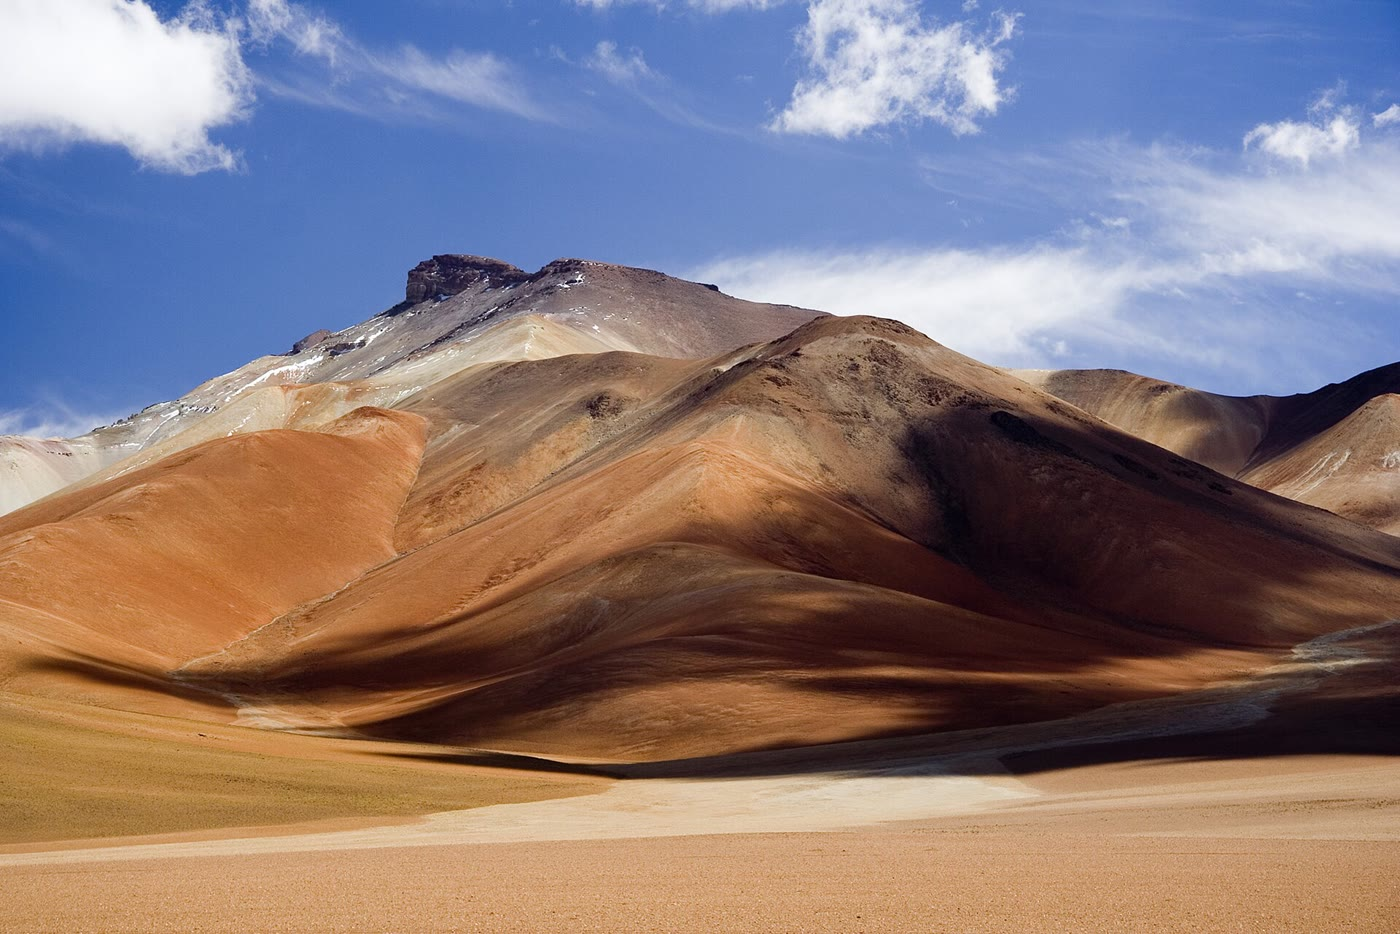
\includegraphics[width=0.66\linewidth]{images/book4/b2-14-altiplano.jpg}
\par\smallskip{\small बोलीविया का आल्टिप्लानो: रेत और बजरी का एक मैदान, नंगी पहाड़ियों की तलहटी में
जिन्हें उनकी चट्टानों ने लाल, गेरुआ और धूसर रंग दिया है। फ़ोटो: Luca Galuzzi, 2006, CC BY-SA 2.5।}
\end{omfigure}
% ledger: gerbault05:andes

\subsection{समतल स्लैब और खोई जड़ें}

स्लैब का कोण स्थिर नहीं है, और सतह पर इसका प्रभाव पड़ता है।

\begin{definition}[समतल-स्लैब क्षेपण]\label{def:b2:himalaya-andes:flat-slab}
\emph{समतल-स्लैब क्षेपण}\index{समतल-स्लैब क्षेपण} वह क्षेपण है जिसमें स्लैब,
अपने पहले अवतरण के बाद, ऊपरी प्लेट के नीचे सैकड़ों किलोमीटर तक लगभग क्षैतिज चलता है
और फिर दोबारा धँसता है।
\end{definition}

एंडीज़ के अनुदिश नाज़्का स्लैब के दो खंड आज समतल हैं: पेरू खंड, जो
लगभग \qty{15}{Ma} से समतल है, और पाम्पा खंड, लगभग \qty{18}{Ma} से। उनके ऊपर
कोई सक्रिय ज्वालामुखी नहीं है। जब पाम्पा स्लैब समतल हुआ, चाप भीतर की ओर खिसका और उसने
कम लावा उगला; समतल खंडों के ऊपर वह शांत हो गया है। पुस्तक 3 का चाप--खाई अंतराल
भीतर की ओर खिसकने की व्याख्या करता है: चाप के नीचे स्लैब जितना मंद होगा, खाई से उतनी ही दूर जाकर
वह उस गहराई तक पहुँचेगा जिस पर कील गलती है; और जो स्लैब उस गहराई के ऊपर समतल बना रहता है वह
गलने के लिए कोई गर्म प्रावार-कील छोड़ता ही नहीं।
% ledger: gauthier24:flat

\begin{definition}[स्थलमंडलीय विस्तरीकरण]\label{def:b2:himalaya-andes:delamination}
\emph{स्थलमंडलीय विस्तरीकरण}\index{स्थलमंडलीय विस्तरीकरण} (डीलैमिनेशन) किसी मोटे हुए स्थलमंडल के निचले भाग का,
यानी उसके प्रावार-स्थलमंडल और कभी-कभी किसी सघन निचली भूपर्पटी का, अलग होकर
दुर्बलमंडल में धँस जाना है, जिसका स्थान गर्म दुर्बलमंडल ले लेता है।
\end{definition}

दक्षिणी पूना के नीचे, \ang{24} और \ang{27}~S के बीच, विस्तरीकरण प्रस्तावित किया गया है,
लगभग 2 से \qty{3}{Ma} पहले, जहाँ युवा मैफ़िक लावा फूटे; और पठार के अनुदिश, भूपर्पटी की
मोटाई और ऊँचाई के परिवर्तनों को ऐसे प्रावार-स्थलमंडल से जोड़ा गया है जो दक्षिणी आल्टिप्लानो के नीचे
पहले ही हट चुका है और मध्य आल्टिप्लानो के नीचे अभी पूरी तरह नहीं। एक
सघन प्रावार-ढक्कन खोने से शेष स्तंभ हल्का हो जाता है: सतह बिना किसी और
लघुकरण के ऊपर उठती है। पूना आल्टिप्लानो से लगभग \qty{1}{km} ऊँचा खड़ा है, लगभग
\qty{11}{km} पतली भूपर्पटी पर, और इस विषमता के लिए या तो हल्की पूना भूपर्पटी चाहिए या उसके
नीचे हल्का प्रावार।
% ledger: gerbault05:delamination, gerbault05:moho

\section{दो पट्टियों की तुलना}\label{sec:b2:himalaya-andes:compared}

दूर से दोनों पठार एक-से दिखते हैं और लगभग हर अन्य बात में भिन्न हैं, जैसा नीचे की तालिका
एकत्र करती है।

\begin{omfigure}
\centering\small
\begin{tabular}{>{\raggedright\arraybackslash}p{0.2\linewidth}|>{\raggedright\arraybackslash}p{0.34\linewidth}|>{\raggedright\arraybackslash}p{0.34\linewidth}}
 & हिमालय और तिब्बत & मध्य एंडीज़ \\ \hline
इंजन & महासागर बंद होने के बाद महाद्वीप बनाम महाद्वीप & किसी महाद्वीप के नीचे धँसती महासागरीय प्लेट \\
अक्ष & \omterm{def:b2:alpine-orogen:ophiolite}{ओफ़ियोलाइटों} वाला सीवन & स्लैब के ऊपर ज्वालामुखी चाप \\
मैग्मावाद & भूपर्पटीय गलित: \omterm{def:b2:crustal-melting:leucogranite}{ल्यूकोग्रेनाइट} & चाप के एंडेसाइट; जहाँ स्थलमंडल खोया वहाँ मैफ़िक लावा \\
अभिसरण & लगभग \qty{45}{mm} प्रति वर्ष, आधा पर्वतमाला में खपता है & लगभग \qty{72}{mm} प्रति वर्ष, अधिकतर क्षेपण में खपता है \\
बड़े भूकंप & MHT पर, असम 1950, $M_w \approx 8.5$ & क्षेपण-अंतरापृष्ठ पर, चिली 1960, $M_w$ 9.5 \\
पठार & माध्य \qty{4.8}{km}, \qty{1180}{km} पर; भूपर्पटी 70--\qty{75}{km} & माध्य \qty{3.8}{km}, \qty{440}{km} पर; भूपर्पटी लगभग \qty{60}{km} \\
पठार की विवर्तनिकी & पूर्व--पश्चिम विस्तारण, बहिर्वेधन & पार्श्वों पर लघुकरण; विस्तरीकरण प्रस्तावित \\
अग्रभूमि & सिंधु-गंगा अग्रगर्त और शिवालिक \omterm{def:b2:alpine-orogen:foreland}{मोलास} & उप-एंडीज़ पट्टी और चाको मैदान \\
\end{tabular}
\par\smallskip{\small दोनों पट्टियाँ साथ-साथ; स्रोत ऊपर के खंडों में उद्धृत हैं,
और चिली का भूकंप 1900 से अब तक अंकित सबसे बड़ा भूकंप है।}
\end{omfigure}
% ledger: lave00:setting, lave00:siwaliks, weinberg16:himalaya, ader12:mht, ader12:quakes, usgs:largest, gerbault05:andes, gerbault05:moho, gerbault05:delamination, nnr56:poles, data:b4-etopo-tibet, data:b4-etopo-andes, cattin01:crust, wang21:rifts, jiao23:extrusion

सबसे गहरा अंतर इसमें है कि नीचे क्या जाता है। एंडीज़ में महासागरीय प्लेट धँसती रहती है, और
अभिसरण का अधिकांश, लगभग \qty{72}{mm} प्रति वर्ष, खाई पर खप जाता है; ऊपरी प्लेट को
कोई 30 मिलियन वर्षों में \qty{310}{km} छोटा करने में उसका केवल लगभग \qty{10}{mm} प्रति
वर्ष लगेगा। हिमालय में कोई हल्की चीज़ देर तक नहीं धँस सकती, इसलिए अभिसरण
ढेर लगाने, मोटा करने और एशिया को एक ओर धकेलने में खर्च होता है। दोनों पट्टियाँ पठार उगाती हैं क्योंकि मोटी भूपर्पटी
ऊँची भूपर्पटी होती है; दोनों पठार तब उठना बंद कर देते हैं जब उनका अपना भार उनके किनारों पर के धक्के को
संतुलित कर देता है, और फिर वे फैलते हैं।
% ledger: nnr56:poles, gerbault05:andes, ader12:mht, jiao23:extrusion

\section{कोई पर्वत कितना ऊँचा हो सकता है?}\label{sec:b2:himalaya-andes:heights}

सबसे ऊँचा शिखर, एवरेस्ट, 2020 में घोषित संयुक्त सर्वेक्षण के अनुसार समुद्र-तल से \qty{8848.86}{m}
ऊपर खड़ा है। बीस किलोमीटर क्यों नहीं? एक मोटी सीमा चट्टान की सामर्थ्य से आती है।

\begin{proposition}[चट्टान की सामर्थ्य से ऊँचाई की एक सीमा]\label{prop:b2:himalaya-andes:height}
घनत्व $\rho$ की चट्टान का एक स्तंभ, जो अपने परिवेश से ऊँचाई $h$ तक खड़ा है और उनके स्तर के ऊपर
कोई पार्श्विक आलंब नहीं रखता, अपने पाद पर ऊर्ध्वाधर प्रतिबल $\rho g h$ और अपने मुक्त पक्षों पर शून्य
क्षैतिज प्रतिबल वहन करता है, अतः अवकल प्रतिबल $\rho g h$। यदि
चट्टान अवकल प्रतिबल $\sigma_d$ पर टूटती है, तो स्तंभ केवल तभी खड़ा रहता है जब $h < \sigma_d/(\rho
g)$ हो।
\end{proposition}

\begin{proof}
स्तंभ के पाद पर ऊर्ध्वाधर प्रतिबल प्रति इकाई क्षेत्रफल ऊपर की चट्टान का भार है,
$\rho g h$। पक्ष मुक्त हैं, अतः वहाँ क्षैतिज प्रतिबल शून्य है। अवकल
प्रतिबल महत्तम और लघुत्तम मुख्य प्रतिबलों का अंतर है, यहाँ $\rho g h - 0$।
विफलता से तभी बचा जा सकता है जब यह $\sigma_d$ से नीचे रहे।
\end{proof}

वास्तविक पर्वत के ढलवाँ पार्श्व उसके क्रोड को थामे रखते हैं, इसलिए उसके नीचे का प्रतिबल
कम होता है; परिमाण की कोटि के रूप में आधा लीजिए, $\rho g h/2$। एवरेस्ट के लिए, $2700 \times 9.8
\times 8849/2 \approx \qty{117}{MPa}$। पुस्तक 3 का बायरली का नियम \qty{200}{MPa} के अभिलंब प्रतिबल के अंतर्गत
किसी भ्रंश पर चट्टान की घर्षण-सामर्थ्य को $50 + 0.6 \times 200 =
\qty{170}{MPa}$ पर रखता है: वही कोटि। तीन गुना ऊँचा पर्वत अपने आधार पर उससे कहीं अधिक भार डालेगा
जितना चट्टान सह सकती है; वह टूटकर फैल जाएगा। पृथ्वी पर आठ से नौ किलोमीटर के शिखर
सीमा के निकट हैं, और पठार, जो अपने शिखरों के टूटने से बहुत पहले फैल जाता है, पाँच पर
स्थिर हो जाता है।
% ledger: tht:everest, byerlee:1975

\section*{अभ्यास}\label{sec:b2:himalaya-andes:exercises}

अभ्यासों के लिए आँकड़े: $g = \qty{9.8}{m.s^{-2}}$; भूपर्पटी और प्रावार के घनत्व
\qty{2700}{kg.m^{-3}} और \qty{3300}{kg.m^{-3}}, जब तक अन्यथा न कहा जाए; सामान्य भूपर्पटी $H =
\qty{35}{km}$।

\begin{exercise}[$\star$]\label{exo:b2:himalaya-andes:1}
एक पठार \qty{3.0}{km} की माध्य ऊँचाई पर खड़ा है।
\cref{prop:b2:himalaya-andes:airy} का उपयोग करके निकालिए (क) उसकी एयरी जड़, (ख) उसकी भूपर्पटी की मोटाई।
(ग) \qty{10}{km} और भूपर्पटी उसे कितना ऊपर उठाएगी?
\end{exercise}

\begin{exercise}[$\star$]\label{exo:b2:himalaya-andes:2}
नेपाल के हिमालय का एक आर-पार भ्रमण गंगा के मैदान से तिब्बत के पठार तक जाता है।
(क) क्रम से वे इकाइयाँ और उन्हें अलग करने वाले भ्रंश लिखिए जिन्हें यह पार करता है। (ख) कौन-सा भ्रंश
सामान्य भ्रंश है? (ग) बृहत् हिमालयी अनुक्रम तक उत्तर की ओर \omterm{def:b2:metamorphic-facies:metamorphism}{कायांतरण} श्रेणी कैसे बदलती है,
और फिर उसके ऊपर?
\end{exercise}

\begin{exercise}[$\star$]\label{exo:b2:himalaya-andes:3}
मध्य नेपाल में \qty{9.2}{kyr} पहले परित्यक्त एक नदी-वेदिका मुख्य अग्र अधिक्षेप के वलनों के आर-पार
\qty{196.5}{m} छोटी हुई है। (क) माध्य लघुकरण-दर
मिलीमीटर प्रति वर्ष में निकालिए। (ख) इसकी तुलना पर्वतमाला के आर-पार GPS अभिसरण,
\qty{17.8}{mm} प्रति वर्ष, से कीजिए। (ग) यह सहमति MFT के उत्तर के भ्रंशों के बारे में क्या बताती है?
\end{exercise}

\begin{exercise}[$\star$]\label{exo:b2:himalaya-andes:4}
हर प्रेक्षण को \omterm{def:b2:himalaya-andes:types}{टक्कर-पट्टी}, \omterm{def:b2:himalaya-andes:types}{एंडीज़-प्रकार की पर्वतजनक पट्टी} या दोनों में रखिए: (क) \omterm{def:b2:alpine-orogen:ophiolite}{ओफ़ियोलाइटों} से
पंक्तिबद्ध एक सीवन; (ख) सक्रिय एंडेसाइटी ज्वालामुखियों की एक पंक्ति; (ग) भूपर्पटी से गले
\omterm{def:b2:crustal-melting:leucogranite}{ल्यूकोग्रेनाइट}; (घ) अग्र के अनुदिश एक गहरी महासागरीय खाई; (ङ) \omterm{def:b2:alpine-orogen:foreland}{मोलास} वाली एक \omterm{def:b2:alpine-orogen:foreland}{अग्रभूमि द्रोणी};
(च) पर्वतमाला के नीचे एक मंद नत भ्रंश पर बड़े भूकंप।
\end{exercise}

\begin{exercise}[$\star\star$]\label{exo:b2:himalaya-andes:5}
हिमालय के आर-पार भारत यूरेशिया के सापेक्ष \qty{45}{mm} प्रति वर्ष की दर से चलता है; नेपाल के आर-पार
पर्वतमाला स्वयं पूर्व में \qty{17.8}{mm} प्रति वर्ष और पश्चिम में \qty{20.5}{mm} प्रति वर्ष सोखती है।
(क) हर स्थिति में पर्वतमाला अभिसरण का कितना अंश लेती है? (ख)
शेष कहाँ जाता है? (ग) \qty{10}{Myr} में शेष भाग कितने लघुकरण के बराबर है?
\end{exercise}

\begin{exercise}[$\star\star$]\label{exo:b2:himalaya-andes:6}
(क) \cref{prop:b2:himalaya-andes:gpe} का उपयोग करके, \qty{3.7}{km} माध्य ऊँचाई वाले
आल्टिप्लानो की अतिरिक्त स्थितिज ऊर्जा निकालिए। (ख) \qty{4.8}{km} पर तिब्बत की ऊर्जा से इसकी तुलना कीजिए।
(ग) दिखाइए कि पतले पठार के लिए, $h \ll H$, $\Delta F$ $h$ के अनुपात में बढ़ता है, और
मोटे पठार के लिए उससे तेज़: इसका किसी पठार की वृद्धि के लिए क्या अर्थ है?
\end{exercise}

\begin{exercise}[$\star\star$]\label{exo:b2:himalaya-andes:7}
(क) $\rho g h/2$ निकालिए, \qty{8848.86}{m} ऊँचे एवरेस्ट के नीचे, $\rho =
\qty{2700}{kg.m^{-3}}$ के साथ। (ख) बायरली के नियम से, $\tau = 0.85\,\sigma_n$ जब अभिलंब प्रतिबल \qty{200}{MPa} से
नीचे हो, और ऊपर $\tau = \qty{50}{MPa} + 0.6\,\sigma_n$; $\tau$ निकालिए, $\sigma_n =
100$ और \qty{200}{MPa} के लिए। (ग) परिमाण की कोटि के उसी नियम से \qty{170}{MPa} की
सामर्थ्य कितनी ऊँचाई की अनुमति देगी?
\end{exercise}

\begin{exercise}[$\star\star$]\label{exo:b2:himalaya-andes:8}
दक्षिणी तिब्बत की दरारें $9 \pm \qty{2}{mm}$ प्रति वर्ष पूर्व--पश्चिम विस्तारण समायोजित करती हैं,
\ang{81} और \ang{92}~E के बीच। (क) \ang{30}~N पर यह खंड कितना चौड़ा है, याम्योत्तर पर प्रति अंश \qty{111.19}{km}
के साथ? (ख) माध्य विस्तारी विकृति-दर, प्रति वर्ष और प्रति सेकंड,
उसके परास के साथ निकालिए। (ग) नेपाल के उत्तर में GPS से मिले $(12.4 \pm 4.7) \times 10^{-9}$ प्रति वर्ष से तुलना कीजिए।
\end{exercise}

\begin{exercise}[$\star\star$]\label{exo:b2:himalaya-andes:9}
नेपाल के नीचे जकड़ा मुख्य हिमालयी अधिक्षेप प्रति वर्ष
\qty{6.6e19}{N.m} का आघूर्ण-घाटा संचित करता है; पिछले 500 वर्षों के भूकंपों ने प्रति वर्ष केवल
\qty{0.9e19}{N.m} मुक्त किया। (क) उन्होंने घाटे का कितना अंश मुक्त किया? (ख) $M_0 =
10^{1.5 M_w + 9.1}$\,\unit{N.m} के साथ, $M_w$ 8.5 के भूकंप का आघूर्ण निकालिए। (ग) घाटे को संतुलित करने के लिए
ऐसे भूकंप कितनी बार आवश्यक होंगे?
\end{exercise}

\begin{exercise}[$\star\star\star$]\label{exo:b2:himalaya-andes:10}
पूना आल्टिप्लानो से \qty{0.7}{km} ऊँचा खड़ा है (4.4 बनाम \qty{3.7}{km}), और उसकी भूपर्पटी
\qty{11}{km} पतली है। आल्टिप्लानो की भूपर्पटी \qty{61.5}{km} मोटी और घनत्व
\qty{2800}{kg.m^{-3}} की लीजिए, और दोनों के नीचे \qty{3300}{kg.m^{-3}} का प्रावार। (क) एक साझा प्रतिपूर्ति-गहराई
के ऊपर दोनों स्तंभों के द्रव्यमानों की समता लिखिए। (ख) यदि अंतर की प्रतिपूर्ति केवल भूपर्पटी करे, तो
पूना भूपर्पटी का घनत्व कितना होना चाहिए, यह निकालिए। (ग) उद्धृत 150 से \qty{200}{kg.m^{-3}} से
तुलना कीजिए, और बताइए कि यह विषमता और किससे समझाई जा सकती है।
\end{exercise}

\begin{exercise}[$\star\star\star$]\label{exo:b2:himalaya-andes:11}
ज्वालामुखी अग्र वहाँ खड़ा होता है जहाँ स्लैब का शीर्ष \qty{105}{km} गहरा है। (क)
\ang{30} पर एकसमान नत स्लैब के लिए, पुस्तक 3 के सूत्र से चाप--खाई अंतराल
निकालिए। (ख) स्लैब अब \ang{30} पर \qty{90}{km} तक नत है, फिर केवल \ang{4} पर:
नया अंतराल और चाप का भीतर की ओर खिसकाव निकालिए। (ग) यदि स्लैब
\qty{95}{km} गहराई पर समतल हो जाए और \qty{300}{km} तक वहीं रहे, तो चाप का क्या होता है?
\end{exercise}

\begin{exercise}[$\star\star\star$]\label{exo:b2:himalaya-andes:12}
अपरदन हिमालय के प्रति किलोमीटर, प्रति मिलियन वर्ष लगभग \qty{300}{km^3} चट्टान हटाता है।
भारत \qty{37.5}{km} मोटी भूपर्पटी \qty{21}{mm} प्रति वर्ष की दर से लाता है। (क) पर्वतमाला के प्रति
किलोमीटर, प्रति मिलियन वर्ष कितनी भूपर्पटी पट्टी में प्रवेश करती है? (ख) अपरदन उसका कितना अंश हटाता है?
(ग) शेष कहाँ हो सकता है?
\end{exercise}

\begin{problem}[{सप्ताहांत समस्या --- दो पठार}]\label{pb:b2:himalaya-andes:1}
इस अध्याय के पट्टी-प्रोफ़ाइल तिब्बत के आर-पार
(\qtyrange{86}{90}{\degree} E) और मध्य एंडीज़ के आर-पार (\qtyrange{19}{21}{\degree} S) बिंदुओं की माध्य ऊँचाई देते हैं।
हर \ang{1.5} अक्षांश और हर अंश देशांतर पर नमूना लेकर, \qty{10}{m} तक पूर्णांकित करने पर, वे
इस प्रकार पढ़े जाते हैं। जब तक अन्यथा न कहा जाए, $g = \qty{9.8}{m.s^{-2}}$, $\rho_c = \qty{2700}{kg.m^{-3}}$,
$\rho_m = \qty{3300}{kg.m^{-3}}$ और सामान्य भूपर्पटी $H = \qty{35}{km}$ मोटी है।

\smallskip
\begin{center}\small
\begin{tabular}{l|ccccccccc}
अक्षांश (\unit{\degree} N) & 26.5 & 28.0 & 29.5 & 31.0 & 32.5 & 34.0 & 35.5 & 37.0 & 38.5 \\ \hline
माध्य ऊँचाई (\unit{m}) & 70 & 5000 & 5030 & 4830 & 5020 & 5150 & 5050 & 4470 & 2210
\end{tabular}

\smallskip
\begin{tabular}{l|cccccccc}
देशांतर (\unit{\degree}) & $-71$ & $-70$ & $-69$ & $-68$ & $-67$ & $-66$ & $-65$ & $-64$ \\ \hline
माध्य ऊँचाई (\unit{m}) & $-3310$ & 970 & 4150 & 3720 & 3740 & 4010 & 3030 & 1170
\end{tabular}
\end{center}
\smallskip

\noindent\textbf{भाग I --- प्रोफ़ाइलों को पढ़ना।}
\begin{enumerate}
\item \qty{3000}{m} से ऊपर के नमूनों को पठार मानकर, तिब्बत की माध्य ऊँचाई
$h_T$ निकालिए, \qty{0.1}{km} तक पूर्णांकित।
\item आल्टिप्लानो के लिए भी यही कीजिए, $h_A$, और आल्टिप्लानो के लिए उद्धृत
\qty{3.7}{km} और पूना के लिए \qty{4.4}{km} की माध्य ऊँचाई से तुलना कीजिए।
\item नमूनों के अनुसार हर पठार कम से कम कितना चौड़ा है (प्रति अंश अक्षांश \qty{111.19}{km};
प्रति अंश देशांतर \qty{104.5}{km}, \ang{20}~S पर)?
\item \ang{26.5} और \ang{28.0}~N के बीच हिमालयी अग्र का माध्य ढलान,
प्रतिशत में, निकालिए।
\item एंडीज़ का प्रोफ़ाइल तिब्बत वाले से इतना अधिक असममित क्यों है?
\end{enumerate}

\noindent\textbf{भाग II --- एयरी मोटाइयाँ।}
\begin{enumerate}[resume]
\item तिब्बत की एयरी जड़ और भूपर्पटी की मोटाई $T_T$ निकालिए, $h_T$ से।
\item आल्टिप्लानो के लिए भी यही कीजिए, $T_A$।
\item भूकंपीय मोटाइयों से तुलना कीजिए, तिब्बत के नीचे 70 से \qty{75}{km} और मध्य आल्टिप्लानो के नीचे 59 से
\qty{64}{km}। कौन-सा अनुमान अधिक दूर है?
\item कौन-सा भूपर्पटीय घनत्व तिब्बत के लिए एयरी की मोटाई को \qty{72.5}{km} के बराबर कर देगा?
\item कौन-सा घनत्व आल्टिप्लानो के लिए \qty{61.5}{km} देगा?
\item भूपर्पटीय घनत्व के अतिरिक्त दो कारण बताइए कि स्थानीय एयरी परिकलन
प्रेक्षित जड़ को क्यों चूक सकता है।
\item भारत के नीचे भूपर्पटी \qty{37.5}{km} मोटी है और तिब्बत के नीचे \qty{72.5}{km}। मोहो पर
\qty{370}{kg.m^{-3}} के घनत्व-अंतर के साथ, बूगेर पट्टी, $\Delta g
= 2\pi G\,\Delta\rho\,t$, से भारत के सापेक्ष तिब्बत की जड़ की बूगेर विसंगति का अनुमान लगाइए, जहाँ $t$
समुद्र-तल के नीचे की अतिरिक्त मोटाई है ($G = \qty{6.674e-11}{m^3.kg^{-1}.s^{-2}}$)। इसकी तुलना
\qty{460}{mGal} के प्रेक्षित अंतर से कीजिए।
\end{enumerate}

\noindent\textbf{भाग III --- आल्टिप्लानो का लघुकरण।} \ang{20}~S पर पठार
\qty{440}{km} चौड़ा है और उसकी भूपर्पटी लगभग \qty{60}{km} मोटी।
\begin{enumerate}[resume]
\item \cref{prop:b2:himalaya-andes:shortening} का उपयोग करके, पुनर्स्थापित चौड़ाई और
आवश्यक लघुकरण निकालिए, यदि भूपर्पटी पहले \qty{35}{km} मोटी थी।
\item संतुलित काटें आल्टिप्लानो में लगभग \qty{50}{km} और
उप-एंडीज़ मंडल में \qty{200}{km} लघुकरण देती हैं। आवश्यक लघुकरण का कितना अंश ग़ायब है?
\item यदि लघुकरण ने अतिरिक्त भूपर्पटी का केवल \qty{55}{\percent} बनाया, तो कितना लघुकरण
आवश्यक है?
\item उप-एंडीज़ पट्टी पतली-त्वचा है। फिर भी उसके लघुकरण को कहीं न कहीं भूपर्पटी को मोटा क्यों करना
ही चाहिए?
\item मान लीजिए भाग III का \qty{314}{km} \qty{30}{Myr} में संचित हुआ। माध्य
दर निकालिए, और आज के नाज़्का--दक्षिण अमेरिका अभिसरण, \qty{72}{mm} प्रति वर्ष, का वह अंश जिसके
यह बराबर है।
\item शेष अभिसरण कहाँ जाता है?
\end{enumerate}

\noindent\textbf{भाग IV --- तिब्बत का भार।}
\begin{enumerate}[resume]
\item $h_T$ के साथ \cref{prop:b2:himalaya-andes:gpe} का उपयोग करके तिब्बत की प्रति इकाई क्षेत्रफल अतिरिक्त स्थितिज
ऊर्जा निकालिए।
\item $h_A$ के साथ आल्टिप्लानो के लिए इसे निकालिए, और दोनों का अनुपात भी।
\item तिब्बत के $\Delta F$ को \qty{100}{km} मोटे स्थलमंडल पर फैलाइए: यह किस माध्य प्रतिबल
के बराबर है?
\item दक्षिणी तिब्बत का विस्तारण, \qty{9}{mm} प्रति वर्ष, \qty{1060}{km} के आर-पार, प्रति वर्ष कितनी
विकृति है?
\item जब भारत अब भी तिब्बत को उत्तर की ओर धकेल रहा है, तब तिब्बत पूर्व--पश्चिम क्यों फैल सकता है?
\item सारांश में: तिब्बत की माध्य ऊँचाई से परिकलित उसकी भूपर्पटी की मोटाई, किलोमीटर तक
पूर्णांकित, बताइए, और भूकंपीय \qty{72.5}{km} का वह अंश जिसकी यह व्याख्या करती है।
\end{enumerate}
\end{problem}
